\documentclass{article}

% The geometry package allows for easy page formatting.
\usepackage{geometry}
\geometry{letterpaper}

% Load up special logo commands.
\usepackage{doc}

% Package for formatting URLs.
\usepackage{url}

% Packages and definitions for graphics files.
\usepackage{graphicx}
\usepackage{epstopdf}
\DeclareGraphicsRule{.tif}{png}{.png}{`convert #1 `dirname #1`/`basename #1 .tif`.png}
%
% Set the title, author, and date.
%
\title{Usability of Security Measures in Ubiquitous Computing Environments}
\author{Joaquin Loustau}
\date{October 16, 2014}

%
% The document proper.
%
\begin{document}

% Add the title section.
\maketitle

% Add an abstract.
\begin{abstract} % JD: I had misrepresented this when I was show LaTeX in class.
The rise of ubiquitous computing ---anytime, everywhere accessible information and communications--- presents new unprecedented scenarios that mean that established usability engineering methodologies, particularly in terms of security measures, have become increasingly out of date. This paper proposes the idea of a new usability for security measures.  The paper suggests that a new security usability must emerge from a fundamental reassessment of existing methods, theories and tools to arrive at an approach that is suitable to a dynamic environment characterized by a myriad of networked processing devices, distributed at all scales throughout life. 
\end{abstract}

% Add various lists on new pages.
\pagebreak
\tableofcontents

% Start the paper on a new page.
\pagebreak

%
% Body text.
%
\section{Introduction}
\label{introduction}
The International Telecommunication Union, a specialized agency of the United Nations (UN) responsible for issues that concern information and communication technologies, reported that the number of mobile-cellular subscriptions will reach almost 7 billion by end 2014, corresponding to a penetration rate of 96\% \cite{itu2014world}. Today, demonstrating the value of ubiquitous computing (ubicomp), the cell phone, or more precisely the “smart phone,” takes center stage crossing a threshold of processor performance, memory capacity and connectivity both cell and local, making it the most widely adopted and ubiquitous computer there has ever been. 

However, the smartphone is just one of several ubiquitous computing devices we encounter during any given day. The future of ubiquitous computing foresees networked microprocessors embedded in everyday objects: not just smart phones and home appliances but furniture, books, sprinklers, etc. ---hundreds of internet-enabled computers communicating to each other over wireless links. 
As the number of ubiquitous computing devices continues to grow, the sheer amount, nature and complexity of the information exchanged will grow exponentially. If the ubicomp systems deployed in our homes, workplaces and vehicles are as vulnerable as today’s personal computers, the implications could be catastrophic. For example, inadequate manipulation of data handled by heart monitors in a clinic or an alarm system for a nuclear power plant could be fatal. The examples are endless. Security is needed to ensure exact and accurate confidentiality, integrity and authentication.

This paper aims to examine the security issues for ubiquitous computing and analyze the usability of the log-in/password mechanism of securing information, along with a brief story of previous works and accomplishments in the corresponding areas. 

\section{Background, Preliminary, and Related Work}
The term ubiquitous computing was coined by Mark Weiser, chief technology officer at Xerox's Palo Alto Research Center (PARC) in 1988 to describe a future in which computers, embedded in everyday objects, replace personal computers (PCs). In his ground-breaking article, ``The Computer for the 21st Century,'' Weiser expresses, ``the most profound technologies are those that disappear. They weave themselves into the fabric of everyday life until they are indistinguishable from it'' \cite{weiser1991computer}.
% JD: Indeed---congratulations on correctly identifying the work that is most widely
%     recognized as the originator of the very concept of ubiquitous computing!

Presently, ubiquitous computing, or ubicomp, is the term given to the third era of modern computing. The first era was defined by the mainframe computer, a single large-time shared computer owned by an organization and used by several individuals at the same time. Second, came the era of the PC, a personal computer predominantly owned and used by one individual, and dedicated to them. Finally, the third and present era, ubiquitous computing, is characterized of small networked computer products, such as smart phones, tablets, and embedded computers built into many of the devices we own ---resulting in a world in which each person owns and uses hundreds of computers a day.

\begin{figure}
  \centering
    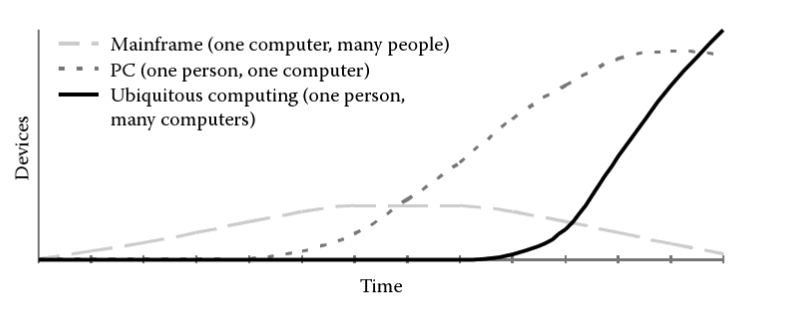
\includegraphics[scale=0.7]{eras_modern_computing}
     \caption{The three eras of modern computing \cite{weiser1991computer}.}
\end{figure}


Rich Gold, a member of Dr.\ Weiser's team at PARC, proposed a taxonomy of properties for ubiquitous computing based on Weiser's formulations. The properties were: sensuous, reactive, communicative, embedded socially and colonizing \cite{gold2007plenitude}. 

In addition to ubiquitous computing, the other major topic that this paper will cover is security. Amoroso \cite{amoroso1994fundamentals} defines computer security as risk management: assessing threats, vulnerabilities and attacks, estimating costs for the threats, estimating probabilities for the attacks given the vulnerabilities, developing appropriate safeguards (a priori vaccines) and countermeasures (a posteriori remedies), and implementing the ones for which the certain price of the defense is worth spending compared to the uncertain loss that a potential threat implies. 

The required characteristics of such secure systems are often summarized in the acronym CIA. This does not refer to the Central Intelligence Agency but is instead a widely used benchmark for evaluation of information systems' security, focusing on the three core goals of \textbf{confidentiality}, \textbf{integrity} and \textbf{availability} of information. Confidentiality refers to limiting information access and disclosure to authorized users. Integrity is the property that refers to the trustworthiness of information resources and is violated whenever information is altered in an unauthorized way. Finally, availability is the property of a system which always ensures that information is accessible when needed. 

The efforts to mitigate the risks of threats to confidentiality, integrity and availability often take the form of user authentication. User authentication is a basic theme in computer security and covers establishing who the user is (identification), verifying this identity (verification), and providing proper access to the resource that the user is allowed to use (authorization). 

This paper will analyze the usability of specific authentication mechanisms, such as the traditional log-in/password schema. It would therefore be desirable to define the term usability in this context. The ISO 9241-11 Guidance on Usability, issued by the International Organization for Standardization, defines usability as: ``the extent to which a product can be used by specified users to achieve specified goals with effectiveness, efficiency and satisfaction in a specified context of use" \cite{iso1998international}.

Usability engineering can be described as the applied side of Human-Computer Interaction (HCI). Building on research in the cognitive-psychology characteristics of users, the human factors of specific hardware and software solutions, and studies of technologies-in-use, usability engineering aims not just to understand interaction issues, but to change practice, improve effectiveness, and make recommendations to improve usability.  

Finally, Nielsen \cite{nielsenusability2012} defines usability as a quality attribute that assesses how easy user interfaces are to use, and is defined by five quality components: learnability, efficiency, memorability, errors and satisfaction. 
% JD: Very comprehensive and well-grounded background!

\section{Methods}
In order to investigate the topic of Usability of Security Measures in Ubiquitous Computing Environments, a top-down approach was employed. Firstly, one performed an exhaustive search of articles, books and journals covering Usability, Security and Ubiquitous Computing as independent concepts. The two main sources chosen for this search were the William H. Hannon Library at Loyola Marymount University and the Association for Computing Machinery's (ACM) Digital Library.  

A narrower and more specific search for materials was then conducted, and sources cited in the selected articles were explored, thus unveiling a myriad of different publications. To assess the reliability of these new sources, Google Scholar was a significantly important tool. Google Scholar provides information such as the number of times the given article has been cited as well as the sources of these citations.  Articles that have been cited time and again and have been published or cited by prestigious scientific journals are most likely to be reliable.

Organizations such as the Association for Computing Machinery (ACM) or the Institute of Electrical and Electronics Engineers (IEEE) are known for their academic rigor, and consequently provide an almost certain guaranty of the credibility and authority of the pieces appearing in their publications. 
% JD: The explicit attention to assessing quality is appreciated here.


\section{Discussion}
While there is extensive bibliography on different strategies to secure information systems, the significantly smaller number of sources available on usability of security measures sheds lights on the fact that the design and usability of user authentication mechanisms is an often overlooked feature of computer systems.

In other words, security and usability seems to be at odds. Yee \cite{yee2004aligning} attributes this conflict to system implementers treating security or usability as an add-on to a finished product. In addition to this, a reason security and usability seem to be opposed is the conflict of interest that exists between the system owner and its users. For example, in the music industry, some implementations of Digital Rights Management (DRM) have caused frustration in genuine customers who would like to play their legally purchased media on different devices and yet are prevented from doing so. 

As people become more connected electronically, the ability to achieve a highly accurate and user-friendly automatic personal identification system is substantially more critical \cite{jain2000biometric}. The usability of security mechanisms is not just a question of improving interfaces to security tools, but designing security to work with the real-world task users perform, and within the physical and social context of that interaction. 

The arising need for procedures that deviate from standard Human-Computer-Interaction (HCI) techniques to evaluate the usability of secure software systems led to the development of a new independent field of study: Human-Computer-Interaction and Security (HCISec). HCISec arose because of the need that was identified HCI experts to improve the usability of secure systems. This need has motivated the research community to re-examine the design and implementation of secure systems \cite{kainda2010security}. However, despite efforts put into this research area, there are still many examples of secure systems being designed without enough consideration of usability.
% JD: Nice find!

The most common and widespread security mechanism, the log-in/password schema, is a clear example of one of such systems. The major user behaviors involved in the log-in/password mechanism are the following:
\begin{enumerate}
\item Visually sighting the dialogue box and the prompts and input field within;
\item Using a pointing device to align the cursor/pointer to the correct location;
\item Homing both hands at the keyboard/touch screen;
\item Entering a string of alphanumeric characters;
\item Clicking on/selecting \textit{OK} or pressing the \textit{ENTER} key \cite{schultz2001usability}.
\end{enumerate}

As can be deduced from observing the previous steps, this approach is most suitable for office situations, where individuals work on a single personal computer for a long period of time ---generally a whole working day. The usability of using a log-in and password for every ubicomp device, however, does not seem clear. 

The number of devices that a user will interact with will require multiple usernames and passwords for the user to remember. Remembering usernames and passwords is difficult even for experienced computer users and typing them in, creates a breakdown in the interaction with the computer, forcing the user to focus on the device rather than on his or her task at hand.  De Alvare and Schultz\cite{dealvare1988framework} discovered that once a password is chosen, a user is unlikely to change it until he/she is aware that it has been compromised. Furthermore, to make memorization easier, users also tend to construct passwords that contain the least amount of characters as possible.

Similarly, mechanisms and policies for increasing the password strength like frequent change of passwords or requesting a password of a certain length that includes different kinds of symbols (See figure 2), often has the opposite effect as users make easy-to-remember passwords and write them down, thereby lowering security \cite{adams1999users}. This shows how a highly secure system from a technical standpoint can be made insecure if the authentication method is difficult or tedious to use. The result is that users find ways to circumvent and shortcut the security system, which leads to vulnerable systems. 

\begin{figure}
  \centering
    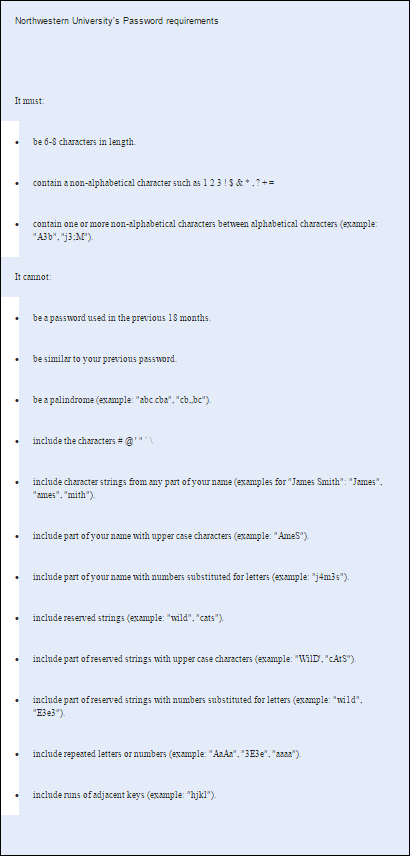
\includegraphics[scale=0.8]{northwestern_password_requirements}
     \caption{Excessive requirements for passwords at Northwestern University \cite{norman2009way}.}
\end{figure}

This clearly correlates to one of the most important usability components: errors.  The log-in/password includes frequent types of expected errors, such as:
\begin{enumerate}
\item Data entry errors;
\item Failure to remember one's password. Password memory is, in fact, the area in which security-usability trade-offs are most likely to occur because the easier the password is to remember, the more likely it is to be guessed or cracked. 
\item Errors resulting from the need to use more than one interaction device, such as homing fingers on the wrong keys on the keyboard, pressing the wrong mouse button. 
\end{enumerate}

Given that errors such as typing in a wrong letter can occur with relative ease, different systems use different criteria to reduce these errors or allow steps to recover from errors. For example, a way to reduce errors, but at the expense of an elevation of security risk, is to allow users to see the password they are typing in, instead of having it masked by asterisks.

The security vulnerabilities and usability issues of the log-in/password call for an alternative to this method that will allow identification of the user with more certainty, probably at the cost of being more difficult to use -decreasing learnability and memorability.

The two alternatives to the log-in/password method often suggested are tokens and biometrics. A security token (also sometimes called authentication token) is a small hardware device that the owner carries to authorize access to a network service. The device may be in the form of a smart card or may be embedded in a commonly used object such as a key fob. 

Security tokens may provide an extra level of assurance through a method known as two factor authentication: the user has a personal identification number (PIN), which authorizes them as the owner of that particular device; the device then displays a number which uniquely identifies the user to the service, allowing them to log in. However, as a physical token, smartcards or other forms of security tokens are subject to be lost or stolen. 

Although smart cards or tokens may improve security through two factor authentication, they certainly entail significant usability hurdles such as complicated user interaction tasks and timing complications (most tokens' pins expire after a given period of time). The learnability of using these artifacts is certainly not comparable to that of the log-in/password approach.  

Biometric identifiers, on the other hand, exploit certain physiological or behavioral characteristics that are distinctive to each person, and thus are more reliable and more capable than knowledge-based and token-based techniques in differentiating between authorized and unauthorized users. By using biometrics system people can be identified by something they \textit{are} instead of something they \textit{have} (e.g., a smart card) or \textit{know} (e.g., their password and log-in). 

There are several steps involved in the use of a biometric authentication method. Consider, for example, a commonly used biometric authentication method, one that reads user fingerprints. Typical user interaction steps include:
\begin{enumerate}
\item Visually sighting a prompt on the display terminal that prompts the user to place a finger on the fingerprint reader;
\item Visually sighting the fingerprint reader;
\item Moving a hand towards the fingerprint reader until it is in close proximity;
\item Rotating the hand until the palm side is down;
\item Extending a finger until it fits over the fingerprint reader;
\item Visually sighting the display terminal for confirmation that the fingerprint read was successful \cite{schultz2001usability}.
\end{enumerate}

An ideal biometric should be \textbf{universal}, where each person possesses the characteristics; \textbf{unique}, where no two people should share the characteristic; \textbf{permanent}, where the characteristic should neither change nor be alterable; and \textbf{collectable}, where the characteristic is readily presentable to a sensor and is easily quantifiable \cite{jain2000biometric}. In practice, however, a characteristic that satisfies all these requirements may not always be feasible for a useful biometric system.

There are eight biometric types that are currently being used in systems: face geometry, fingerprint, hand geometry, iris pattern, retinal pattern, signature, voice print, and facial thermogram. Even though it is being `marketed' as a new user-friendly user authentication mechanism, there is little research so far into the usability of these systems. Most work and research on biometric systems focus on security and accuracy. 

A traditional way of testing a biometric system is to measure the correlation between the false-acceptance rate (FAR) ---the percentage of unauthorized users incorrectly matched to a valid user's biometric--- and the false-rejection rate (FRR) ---the percentage of incorrectly rejected valid users. Biometric specialists normally agree that the biometric rates of FAR and FRR are the equivalent of the password space in PIN/Password based authentication \cite{biometrics2003biometrics}. Biometrics do not provide perfect (unique) identification. The matching process is probabilistic and is consequently subject to statistical error.    The UK Government Biometrics Working Group (BWG) expressed in their “Biometric Security Concerns” that current knowledge of biometric algorithm behavior and human feature randomness and variation does not permit theoretical analysis of biometric system performance \cite{biometrics2003biometrics}.

Such as with the log-in/password approach, the main usability problem with a biometric mechanism is that it is prone to certain errors, such as:
\begin{enumerate}
\item Failure to place a finger in the proper position in the fingerprint reader;
\item Placing the ``wrong" finger (i.e., a finger with a cut, which is likely to render the fingerprint read invalid) in the fingerprint reader;
\item Failure to keep finger still enough to have the fingerprint read;
\end{enumerate}

The aforementioned security measures display a problem common to most security definitions: they focus on attackers ---agents with a malicious intent--- rather than on legitimate users of a system. The problem with concentrating on invalid users or attackers/hackers is that it ignores the fact that non-malicious users may also compromise the system as the result of a poorly designed system.  Security mechanisms that omit usability may lead users to perceive an action as harmless when it is not or mistakenly encourage users to engage in an insecure interaction. 

The key to finding an appropriate security mechanism for an ubicomp environment should consequently not focus so much on the technical aspect but should instead have usability as a primary motivation or goal.  Zurko and Simon \cite{zurko1996user} refer to this approach as \textbf{user-centered security}, and one subscribes to this concept. 

As already mentioned, the traditional log-in/password schema completely disrupts a smooth flow of work in the settings prescribed by a ubiquitous computing environment. As users abandon a static room with its desktop computer for a world in which every device offers computer support, the aspects of mobility, cooperation, interruption, and sharing of material become core aspects of much real world work. The design of security systems for this kind of working environments needs to accommodate such challenges, rather than unconsciously adopt existing user authentication mechanisms.

Historically, the first security application to articulate a user-centered design philosophy was Privacy-Enhanced Mail (PEM) \cite{linn1993privacy}. ``The set of supported measures offers added value to users, enhancing rather than restricting the set of capabilities available to users." This was a startling vision in the security community that largely perceived security requirements as watching and restricting users. While usability problems with the certificate authority infrastructure kept PEM from being widely deployed, its primary motivation to offer users desirable security services such as privacy for their daily electronic mail remains a laudable goal still  unmet today \cite{zurko1996user}.  This example shows that considerations for users' natural working patterns rather than more complex techniques can strengthen the security of the system.

While the implementation details of a suitable security mechanism for an ubicomp environment may vary (although automation appears to be the key), one believes any security mechanism designed for this kind of environment should succeed in accomplishing the following five objectives:

\begin{enumerate}
 \item \textbf{Allow for proximity-based user authentication.}\\
 The term proximity-based user authentication was first introduced by Jakob E. Bardram \cite{bardram2005trouble} in his article based on Donald Norman's essay ``The Trouble with UNIX" \cite{norman1981trouble}. The need for short, fast interaction with ubicomp devices without focus shifts or breakdowns in current processes requires security measures that do not imply a significant interruption to the user. A proximity-based user authentication would just require the user to be within a determined distance of the device to be recognized and logged in. A possible way to implement this could stem from biometrics systems. 
 
 \item \textbf{Support migrating user session within devices.}\\
 There is a class of ubicomp devices designed to accompany users through different tasks and in changing contexts and environments. Suppose a user connects with his alarm clock/music player in the morning and selects his music play list. It would be desirable for the user to be able to easily migrate his current session to the kitchen audio system as he eats breakfast, then to his car stereo as he drives to work and finally to his cellphone as he walks from the parking lot to his office. Ubiquitous devices should allow for users to easily activate their session when switching devices without having to start the authentication process all over again. 
 
 \item \textbf{Easy transition between users in the same device/allow multi-user sessions.}\\
 Ubiquitous computing involves ``computerizing" everyday devices. Some of these devices are used by multiple users quasi-simultaneously in their present state, and therefore would need to accommodate for a quasi-simultaneous use of its ``computing capacities" in a ubicomp environment. Easily exchangeable sessions within the same device would be the answer to this.
 
 \item \textbf{Flexibility to create and/or delete new users (for users authorized to do so).}\\
 It should be as easy and clear as possible for system administrators to be able to add or delete users that no longer should have access to certain devices or that are no longer par of the company, organization, family, etc.  Deleting or adding new users should by no means affect any previous or current information from other existing users.

 \item \textbf{Common procedures and interfaces within devices when deemed possible.}\\
 ``As new technologies penetrate our lives at an increasing rate, we no longer know what functionality to expect from our refrigerator, our television, our car, our heating control system, and so forth. There is a trend towards product integration and we see an increased complexity of especially domestic technology" \cite{petersen2002usability}.
 % JD: This direct quote is too long---better to paraphrase this.
The characteristics of a ubiquitous computing environment call for a unified interface within devices in order to assist user learnability, as the user continuously encounters new devices. Logically, the interface used for the equipment in a hospital room or nuclear reactor and that used by a refrigerator will unlikely be similar in content, capabilities, security, etc. However, the designers of the `devices of the future' should elaborate a unique set of design guidelines for ubicomp devices and try to be consistent with them to as much extent as possible. 
\end{enumerate}

These characterictiscs briefly summarize what one believes should define the design of usable security measures for a ubiquitous computing environment.  

Needless to say, any security measure designed should also be consistent with usability principles and guidelines, and offer enhanced interaction protocols and interfaces with better feedback, and the development and continual communication to support the development of appropriate conceptual models. 


\section{Conclusions}
As user-interface technology continues to evolve and users' needs continue to diversify at an unprecedented pace, no single technology or architecture is always ``user friendly." 

The present status quo and prospects of a world in which every device has a computer embedded in it urge us to produce systems that are more secure, that enhance privacy, and that are still eminently usable. 

The paradigm to achieve this should be the full integration of security and usability concerns into the software development process, thus enabling developers to build secure systems that work in the real world \cite{flechais2003bringing}. Despite what is commonly believed, security and usability may, and in fact, should be considered jointly as they affect each other --- usability factors can cause users to behave insecurely, and security factors may obviously impair performance.

After analyzing the security and usability of the most common authentication method ---log-in/password--- and two alternatives to it usually offered, one set out to outline the requirements of new security measures in ubiquitous computing environments.

These requirements take the form of three steps. Firstly, appropriate technologies, probably including automation, will need to be developed. Secondly, a design with the following characteristics must be constructed: allows for proximity-based user authentication, supports migrating user session within devices, allows multi-user sessions, enables flexible creation and deletion of users, and lastly follows a common standard designs with other ubiquitous devices. Finally, new security measures developers must seek to obtain continual communication from users to support the development of appropriate conceptual models.

\bibliography{assignment1016}
\bibliographystyle{plain}

\end{document}
